\documentclass[11pt,a4paper,reqno]{amsart}

\usepackage[utf8]{inputenc}
\usepackage[T1]{fontenc}
\usepackage{lmodern}
\usepackage{amsmath,amssymb,amsthm}
\usepackage{graphicx}
\usepackage{booktabs}
\usepackage{array}
\usepackage[margin=28mm]{geometry}
\usepackage{xurl}
\usepackage[hidelinks]{hyperref}
\usepackage{orcidlink}
\usepackage{microtype}

\newtheorem{theorem}{Theorem}[section]
\newtheorem{proposition}[theorem]{Proposition}
\newtheorem{lemma}[theorem]{Lemma}
\newtheorem{corollary}[theorem]{Corollary}
\newtheorem*{conjTwo}{Conjecture 2}
\newtheorem*{conjSix}{Conjecture 6}
\newtheorem*{theoremW}{Theorem W}
\theoremstyle{remark}
\newtheorem{remark}[theorem]{Remark}

\numberwithin{equation}{section}

\newcommand{\one}{\mathbf{1}}
\newcommand{\T}{\mathsf{T}}
\newcommand{\hc}{\operatorname{hc}}
\newcommand{\Hess}{\operatorname{Hess}}
\newcommand{\artanh}{\operatorname{artanh}}
\newcommand{\cT}{\mathcal{T}}
\newcommand{\cR}{\mathcal{R}}
\newcommand{\C}{\mathbb{C}}
\newcommand{\Z}{\mathbb{Z}}
\newcommand{\E}{\mathbb{E}}

\title[Two conjectures of Wormald on Hamilton cycles]{Two conjectures of Wormald on Hamilton cycles in tournaments}

\author{Deep Bhattacharjee\,\orcidlink{0000-0003-0466-750X}}
\address{Formerly, Electro-Gravitational Space Propulsion Laboratory (EGSPL), Bhubaneswar, Odisha 751030, India}
\address{Formerly, University of Calcutta, Senate House, 87/1 College Street, Kolkata 700073, West Bengal, India}
\email{d.bhattacharjee@erl-forschung.de}
\email{itsdeep@live.com}
\email{egspl@proton.me}
\thanks{\sloppy Corresponding author: Deep Bhattacharjee. Email: \href{mailto:d.bhattacharjee@erl-forschung.de}{d.bhattacharjee@erl-forschung.de}, \href{mailto:itsdeep@live.com}{itsdeep@live.com}, \href{mailto:egspl@proton.me}{egspl@proton.me}; ORCID \href{https://orcid.org/0000-0003-0466-750X}{0000-0003-0466-750X}.}

\subjclass[2020]{05C20; 05C45; 05C50; 05C80; 15A15}
\keywords{tournament; Hamilton cycle; random blow-up; skew-symmetric matrix}
\date{26 October 2026}

\begin{document}

\begin{abstract}
\itshape
A tournament is a complete graph in which every edge has been given a direction, and a Hamilton cycle in it is a directed cycle through all the vertices. Let $h(n)$ be the largest number of Hamilton cycles that a tournament on $n$ vertices can have, and let $g(n)=2^{-n}(n-1)!$ be the expected number of Hamilton cycles of a random tournament on $n$ vertices. Wormald obtained lower bounds for $h(n)$ by replacing every vertex of a fixed regular tournament $T$ on $d$ vertices by a random tournament on $n$ vertices. The expected number of Hamilton cycles of the result is governed by a number $H$, the determinant of the Hessian of a function defined implicitly by $T$; the bound is $\sqrt{d/H}\,g(dn)$, or $e^{1/d}\sqrt{d/H}\,g(dn)$ when the blocks are regular. Wormald computed $H$ for a few small tournaments, found that $d/H$ was the square of a rational number every time, and could not explain it. We prove that $H=d\det(d^2I+S^2)/\det(d^2I-S^2)$, where $S$ is the skew adjacency matrix of $T$, so that $H\neq0$ and $\sqrt{d/H}=\det(dI-S)/\det(dI-iS)$ is a ratio of two positive integers. This is his Conjecture~6. For the cyclic tournament on $d$ vertices the formula becomes $\sqrt{d/H}=\bigl((d+1)^d+(d-1)^d\bigr)/\bigl((d+i)^d+(d-i)^d\bigr)$, which tends to $\cosh1/\cos1=2.8559578925\ldots$ as $d$ grows. This is his Conjecture~2, and it identifies the constant $2.855958$ that he estimated by fitting polynomials; it also explains why the terms in $1/d$ and $1/d^3$ of his fits were nearly zero. We add bounds for $\sqrt{d/H}$ over all regular tournaments on $d$ vertices, with equality in the lower bound exactly for doubly regular tournaments. Every statement is proved by hand.
\end{abstract}

\maketitle



\medskip
\begin{quote}
\small\sloppy
\noindent\textbf{Note.} The results of this paper were first made public on 14 October 2026, as release \texttt{v1.0.0} of the repository \url{https://github.com/creelie/Breakthrough-problems-1}; later versions of that repository (\texttt{v1.0.1} of 22 October and \texttt{v1.1.0} of 25 October) are archived on Zenodo as \href{https://doi.org/10.5281/zenodo.23567153}{10.5281/zenodo.23567153} and \href{https://doi.org/10.5281/zenodo.23631103}{10.5281/zenodo.23631103} (concept DOI \href{https://doi.org/10.5281/zenodo.23567152}{10.5281/zenodo.23567152}). An earlier and incomplete version of the paper appeared on Hexagon on 22 October 2026 as the preprint \texttt{hexagon:2610.00460}, available at \url{https://hexagonmath.org/2610.00460}. That version relied on a computer certificate and on computer checks for part of its evidence, carried a verification section, and left the scope of some statements unstated. This version is complete and self-contained: every statement is proved by hand, the scope of each result is stated, the only unrefereed sources it depends on are the paper of Wormald that states the conjectures and the two later works named next, and no statement rests on a computer. Two works posted after 14 October 2026 overlap with this one and are acknowledged here. Divoux and Wang (arXiv:2610.23755, 16 October 2026) prove, by a different method, that $h(n)\sim(\cosh1/\cos1)\,g(n)$, which is Wormald's Conjecture~5 and is stronger than the lower bound of Corollary~\ref{cor:hn}; their Proposition~7.1 is used in Section~\ref{sec:intro} for one comparison and nowhere else. Liu and Ye (\url{https://github.com/LStar404/wormald-tournament-conjectures}, first posted 19 October 2026) treat Wormald's Conjectures~1, 2 and~6 independently. The source of this revision is in the repository \url{https://github.com/creelie/Paper_8}, release \texttt{v1.0.0}, archived on Zenodo as \href{https://doi.org/10.5281/zenodo.23659586}{10.5281/zenodo.23659586} (concept \href{https://doi.org/10.5281/zenodo.23659585}{10.5281/zenodo.23659585}), together with programs that recompute the table and the numerical values of the paper.
\end{quote}

\section{Introduction}\label{sec:intro}

Let $\hc(T)$ be the number of Hamilton cycles of a tournament $T$, let $h(n)$ be the largest value of $\hc$ over tournaments on $n$ vertices, and let $g(n)=2^{-n}(n-1)!$ be the expected number of Hamilton cycles of a uniformly random tournament on $n$ vertices.\footnote{A tournament on $n$ vertices has $\binom n2$ arcs, one for each pair of vertices, each of which may point either way; a uniformly random tournament chooses every direction independently with probability $1/2$. A given cyclic order of the $n$ vertices is a Hamilton cycle with probability $2^{-n}$, and there are $(n-1)!$ cyclic orders, which gives $g(n)$.} The random tournament shows that $h(n)\ge g(n)$, an argument that goes back to Szele~\cite{Sz} for Hamilton paths. Alon~\cite{Al} proved $h(n)=O(n^{3/2}g(n))$, and Friedgut and Kahn~\cite{FK} lowered the exponent below $5/4$. On the side of constructions, Adler, Alon and Ross~\cite{AAR} found tournaments with $(e-o(1))g'(n)$ Hamilton paths, where $g'(n)=2^{1-n}n!$ is the expected number of Hamilton paths of a random tournament. Divoux and Wang~\cite{DW} have since found the global asymptotic $h(n)=(\cosh1/\cos1+o(1))g(n)$ and the analogous result for Hamilton paths. The exact calculation of this paper is carried out directly from Wormald's definition and does not use that asymptotic.

Wormald~\cite{W} improved the constant $e$ by averaging over random blow-ups of a fixed tournament. Let $T$ be a tournament on $[d]=\{1,\dots,d\}$ with $d$ odd. The random tournament $\cT(T,n)$ on $dn$ vertices is obtained by replacing each vertex $j$ of $T$ by an independent uniformly random tournament $T_j$ on $n$ vertices and each arc $jk$ of $T$ by all arcs from $T_j$ to $T_k$; in $\cR(T,n)$ the $T_j$ are uniformly random \emph{regular} tournaments ($n$ odd).\footnote{A tournament is regular when every vertex has the same number of out-neighbours, which forces an odd number of vertices and out-degree $(d-1)/2$.} See Figure~\ref{fig:blowup}. When $T$ is regular, Wormald's main results~\cite[Theorems~1 and~4]{W} read as follows.

\begin{theoremW}
Let $T$ be a regular tournament on $d\ge3$ vertices with adjacency matrix $A$. Put $M(y)=I-(\tfrac12I+A)\operatorname{diag}(y_1,\dots,y_d)$, $K(y)=\det M(y)$ and $z=2/d$. Then $K(z,\dots,z)=0$ and $\partial K/\partial y_d\neq0$ there, so $K(y)=0$ defines an analytic function $y_d=h(y_1,\dots,y_{d-1})$ near $(z,\dots,z)$. Let $H$ be the determinant of the Hessian at $\theta=0$ of
\[
\tilde f(\theta_1,\dots,\theta_{d-1})=\log h\bigl(ze^{i\theta_1},\dots,ze^{i\theta_{d-1}}\bigr).
\]
If $H\neq0$, then, as $n\to\infty$,
\[
\E\,\hc(\cT(T,n))\sim\rho_\cT(T)\,g(dn)\quad\text{and}\quad \E\,\hc(\cR(T,n))\sim\rho_\cR(T)\,g(dn),
\]
where $\rho_\cT(T)=\sqrt{d/H}$ and $\rho_\cR(T)=e^{1/d}\rho_\cT(T)$.
\end{theoremW}

Wormald computed $H$ with a computer algebra system for several small tournaments, among them the cyclic tournament $R_d$, which has an arc from $j$ to $j+r$ modulo $d$ for $1\le r\le (d-1)/2$, and he found $\rho_\cR(R_{101})=2.855883\ldots$. Since a random tournament from $\cR(T,n)$ has at least its expected number of Hamilton cycles with positive probability, this gives $h(n)>2.85588\,g(n)$ for infinitely many $n$. He noted that it is unexplained why $d/H$ was a perfect square in every example, and made the following conjectures~\cite[Conjectures~2 and~6]{W}.

\begin{conjTwo}[Wormald]
The limit $\lim_{d\to\infty}\rho_\cR(R_d)$, over odd $d$, exists.
\end{conjTwo}

\begin{conjSix}[Wormald]
For every regular tournament on $d\ge3$ vertices, $H\neq0$ and $d/H$ is the square of a rational number.
\end{conjSix}

By fitting polynomials in $1/d$ to his values for $d\le101$, Wormald estimated the limit in Conjecture~2 as $2.8559579$, and he observed that the coefficients of $1/d$ and of $1/d^3$ in the fit were nearly zero while that of $1/d^5$ was not. He also conjectured that this constant is $\lim h(n)/g(n)$~\cite[Conjecture~5]{W}.

We prove both conjectures by computing $H$ in closed form. For a tournament with adjacency matrix $A$ let $S=A-A^\T$ be its skew adjacency matrix: $S_{jk}=1$ if $jk$ is an arc, $S_{jk}=-1$ if $kj$ is an arc, and $S_{jj}=0$.

\begin{theorem}\label{thm:main}
Let $T$ be a regular tournament on $d\ge3$ vertices with skew adjacency matrix $S$, and let $0,\pm i\mu_1,\dots,\pm i\mu_m$ $(m=(d-1)/2,\ \mu_k\ge0)$ be the eigenvalues of $S$. Then
\begin{equation}\label{eq:main}
H=d\,\frac{\det(d^2I+S^2)}{\det(d^2I-S^2)}.
\end{equation}
Here $\det(d^2I-S^2)=\det(dI-S)^2$ and $\det(d^2I+S^2)=\det(dI-iS)^2$, where $\det(dI-S)$ and $\det(dI-iS)$ are positive integers, and
\begin{equation}\label{eq:rho}
\rho_\cT(T)=\sqrt{\frac dH}=\frac{\det(dI-S)}{\det(dI-iS)}=\prod_{k=1}^m\frac{d^2+\mu_k^2}{d^2-\mu_k^2}.
\end{equation}
\end{theorem}

\begin{corollary}\label{cor:conj6}
Conjecture~6 holds.
\end{corollary}

For the cyclic tournament everything is explicit.

\begin{theorem}\label{thm:cyclic}
Let $d\ge3$ be odd and let $S$ be the skew adjacency matrix of $R_d$. Then $\det(xI-S)=\tfrac12\bigl((x+1)^d+(x-1)^d\bigr)$, and
\begin{equation}\label{eq:cyclic}
\rho_\cT(R_d)=\frac{(d+1)^d+(d-1)^d}{(d+i)^d+(d-i)^d}
=\Bigl(\frac{d^2-1}{d^2+1}\Bigr)^{d/2}\frac{\cosh\bigl(d\artanh\frac1d\bigr)}{\cos\bigl(d\arctan\frac1d\bigr)}.
\end{equation}
Consequently
\[
\lim_{d\to\infty}\rho_\cR(R_d)=\lim_{d\to\infty}\rho_\cT(R_d)=\frac{\cosh 1}{\cos 1}=2.85595789256511371\ldots,
\]
and $\rho_\cR(R_d)=\dfrac{\cosh1}{\cos1}\Bigl(1-\dfrac{\tan1-\tanh1}{3d^2}+O(d^{-4})\Bigr)$. In the expansion of $\rho_\cR(R_d)$ in powers of $1/d$ the coefficients of $d^{-1}$ and $d^{-3}$ vanish and that of $d^{-5}$ equals $-\cosh1/(3\cos1)$.
\end{theorem}

So Conjecture~2 holds, its limit is the constant $2.855958$ of Wormald's Conjecture~5, and the last statement accounts for the pattern he saw in his fits. The first expression in \eqref{eq:cyclic} reproduces every exact value in his table, from $\rho_\cT(R_3)=2$ and $\rho_\cT(R_5)=44/19$ to $\rho_\cT(R_{13})=41637757888/15769379963$.\footnote{Wormald remarks that extrapolating the exact values may be hard, citing the factorisation $53\cdot297535471$ of the denominator for $d=11$. That number is the denominator for $d=13$; for $d=11$ it is $41833969=43\cdot307\cdot3169$.} Combined with Theorem~W, Theorem~\ref{thm:cyclic} gives a lower bound for $h(n)$.

\begin{corollary}\label{cor:hn}
$\limsup_{n\to\infty}h(n)/g(n)\ge\cosh1/\cos1$. The same holds for the largest number $h'(n)$ of Hamilton paths in a tournament on $n$ vertices, with $g'$ in place of $g$.
\end{corollary}

Theorem~\ref{thm:main} also turns questions about $\rho_\cT$ into questions about the spectrum of $S$. Wormald's Conjecture~1 asks whether $R_d$ maximises $\rho_\cT$ among tournaments on $d$ vertices; among regular ones we obtain the following bounds, and $\cosh1/\cos1$ turns out to lie within $0.051\%$ of the best value that blow-ups of regular tournaments can give.

\begin{theorem}\label{thm:bounds}
Let $T$ be a regular tournament on $d\ge3$ vertices and $m=(d-1)/2$. Then
\[
\Bigl(\frac{d+1}{d-1}\Bigr)^{m}\le\rho_\cT(T)\le U_d,
\]
with equality on the left if and only if $T$ is doubly regular. Here, with $\sigma=\cot^2\frac{\pi}{2d}$, $q=\lfloor d(d-1)/(2\sigma)\rfloor$ and $r=d(d-1)/2-q\sigma$,
\[
U_d=\Bigl(\frac{d^2+\sigma}{d^2-\sigma}\Bigr)^{q}\,\frac{d^2+r}{d^2-r},
\]
and
\[
\lim_{d\to\infty}U_d=\frac{(\pi^2+4)(3\pi^2-8)}{(\pi^2-4)(\pi^2+8)}=2.8574011776\ldots.
\]
In particular $\rho_\cR(T)>e$ for every regular tournament $T$, and every limit point of $\max_T\rho_\cR(T)$, the maximum over regular tournaments on $d$ vertices, lies in $[2.8559578,\,2.8574012]$.
\end{theorem}

Divoux and Wang~\cite[Proposition~7.1]{DW} give a sharper universal bound for $Z(K)=\det(I-K)/\det(I-iK)$. For $K=S/d$ with odd $d$ their bound is exactly the first expression in \eqref{eq:cyclic}, so with \eqref{eq:rho} it shows that $R_d$ maximises $\rho_\cT$ among regular tournaments on $d$ vertices. Theorem~\ref{thm:bounds} is an elementary spectral estimate with a self-contained proof; it is not the sharpest bound known. Nothing proved here uses their asymptotic result.

A tournament is doubly regular if every two vertices have the same number, necessarily $(d-3)/4$, of common out-neighbours; such tournaments exist exactly when there is a skew Hadamard matrix of order $d+1$~\cite{RB}, for instance for the quadratic residue tournaments of prime order $d\equiv3\pmod 4$.\footnote{The quadratic residue tournament on the field with $d$ elements has an arc from $a$ to $b$ when $b-a$ is a nonzero square; for $d\equiv3\pmod4$ the element $-1$ is not a square, so exactly one of $b-a$ and $a-b$ is a square and this is a tournament.} For $d\le9$ an enumeration of all regular tournaments shows that $R_d$ maximises $\rho_\cT$ among regular tournaments (Table~\ref{tab:small}); the upper bound $U_d$ is within $10^{-4}$ of $\rho_\cT(R_d)$ there.

\begin{remark}\label{rem:circulants}
Wormald also lists values of $\rho_\cT$ for seven $9$-vertex circulants, the digraphs with an arc $jk$ whenever $k-j\bmod 9$ lies in a set $D$ of size four, and from the smallest of them, $1.4582$ for $D=\{1,3,4,5\}$, he infers that some regular $n$-tournaments have at most about $1.4582\,e^{1/9}g(n)\approx1.63\,g(n)$ Hamilton cycles. Only one of the seven sets, $D=\{1,2,3,5\}$, defines a tournament: each of the other six contains both $r$ and $9-r$ for some $r$, so its circulant has $2$-cycles and Theorem~W does not apply to it. For $D=\{1,2,3,5\}$ Theorem~\ref{thm:main} gives $\rho_\cT=451696/183937=2.4557\ldots$, matching his value. By Theorem~\ref{thm:bounds} every regular tournament on $9$ vertices has $\rho_\cT\ge(5/4)^4=2.4414\ldots$, and blow-ups of regular tournaments never give fewer than $(e-o(1))g(n)$ expected Hamilton cycles. The bound $1.63\,g(n)$ is therefore not supported by these examples.
\end{remark}

The proof of Theorem~\ref{thm:main} has two parts. Proposition~\ref{prop:hessian} identifies Wormald's analytic $H$, the Hessian determinant of an implicit function, with the determinant of an explicit matrix built from $S$; this is done by a Schur complement and a second-order expansion. The rest is the algebra of skew-symmetric matrices. The determinantal and enumerative bookkeeping is of the same kind as in the author's earlier work on counts attached to group actions and finite complexes~\cite{Bha22a,Bha22b,BB26}.

\begin{figure}[t]
\centering
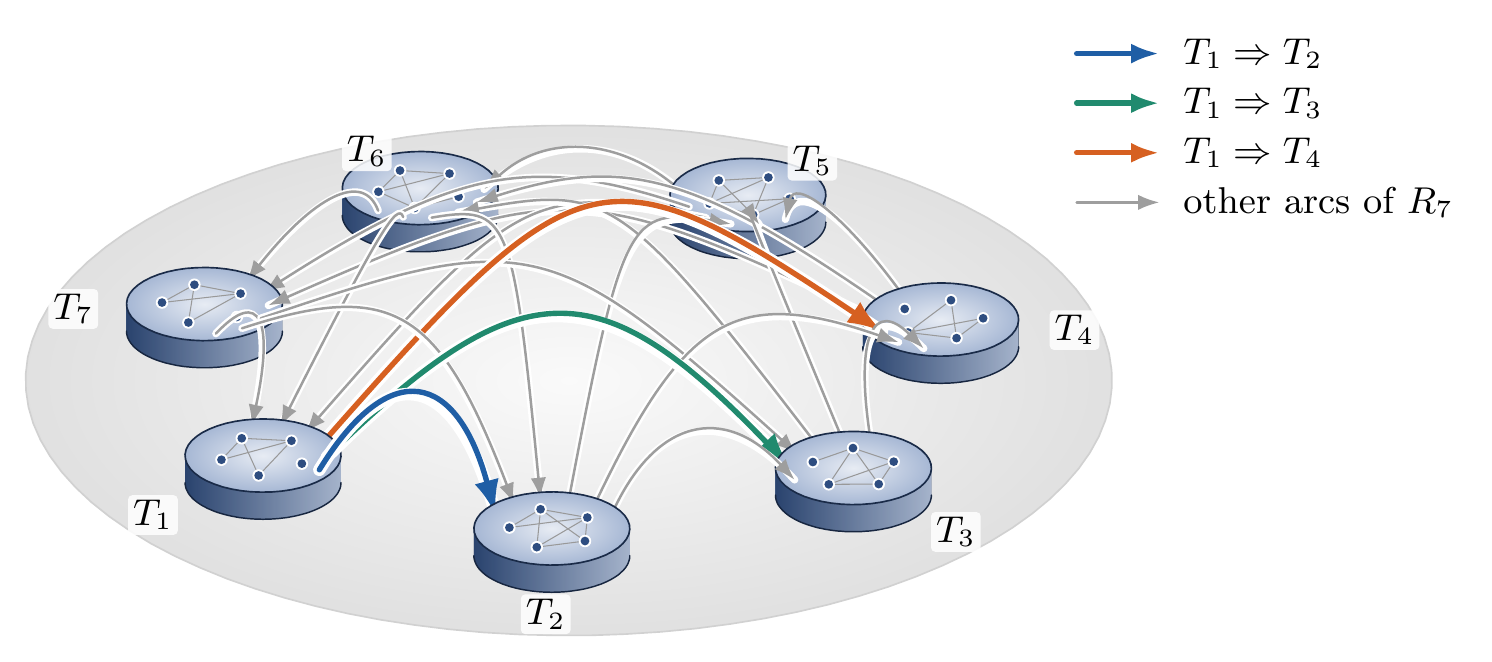
\includegraphics[width=0.82\textwidth]{figures/blowup.png}
\caption{The random blow-up $\cT(R_7,n)$. Each vertex $j$ of the cyclic tournament $R_7$ becomes a random tournament $T_j$ on $n$ vertices, and every arc of $R_7$ becomes the complete set of arcs from one block to the next; the three arcs leaving $T_1$ are coloured and the other eighteen are grey.}
\label{fig:blowup}
\end{figure}

\section{Preliminaries}\label{sec:prelim}

Throughout, $T$ is a regular tournament on $[d]$ with $d=2m+1\ge3$, $A$ is its adjacency matrix and $S=A-A^\T$. We write $J$ for the all-ones matrix, $\one$ for the all-ones vector, $I$ for the identity and $e_j$ for the standard basis vectors. Regularity means $A\one=A^\T\one=m\one$. Since $A+A^\T=J-I$,
\begin{equation}\label{eq:IA}
I+2A=J+S,\qquad S\one=0,\qquad \one^\T S=0.
\end{equation}

\begin{lemma}\label{lem:N}
Let $N=(I+2A)/d$, $P=J/d$ and $Y=S/d$. Then $N=P+Y$, $N\one=\one$, $\one^\T N=\one^\T$, $P^2=P$ and $PY=YP=0$. The matrix $Y$ is real and skew-symmetric, every eigenvalue of $S$ has modulus at most $d-1$, and $I\pm Y$ and $I-Y^2=(I-Y)(I+Y)$ are invertible.
\end{lemma}

\begin{proof}
Everything except the last two statements follows from \eqref{eq:IA}. Each row of $S$ has $d-1$ entries $\pm1$, so by Gershgorin's theorem the eigenvalues of $S$, which are purely imaginary, have modulus at most $d-1$.\footnote{A real skew-symmetric matrix is normal with purely imaginary eigenvalues, and Gershgorin's theorem places every eigenvalue in a disc centred at a diagonal entry, here $0$, with radius the sum of the absolute values of the other entries of its row.} The eigenvalues of $I\pm Y$ are $1\pm i\mu/d$ with $\mu$ real, hence nonzero.
\end{proof}

The second lemma restricts a determinant to the hyperplane $x_1+\dots+x_d=0$. Let $E$ be the $d\times(d-1)$ matrix whose $j$-th column is $e_j-e_d$.

\begin{lemma}\label{lem:border}
If $F$ is a $d\times d$ matrix over a field of characteristic $0$ with $F\one=\one$ and $\one^\T F=\one^\T$, then $\det(E^\T FE)=d\det F$.
\end{lemma}

\begin{proof}
Let $Q=(E\mid\one)$. Since $E^\T\one=0$, $F\one=\one$ and $\one^\T F=\one^\T$,
\[
Q^\T FQ=\begin{pmatrix}E^\T FE&E^\T\one\\ \one^\T E&\one^\T\one\end{pmatrix}=\begin{pmatrix}E^\T FE&0\\0&d\end{pmatrix},
\]
so $(\det Q)^2\det F=d\det(E^\T FE)$. For $F=I$ this reads $(\det Q)^2=d\det(E^\T E)=d\det(I+J_{d-1})=d^2$, because $I+J_{d-1}$ has the eigenvalue $d$ once and the eigenvalue $1$ with multiplicity $d-2$. Comparing the two identities gives the claim.
\end{proof}

\section{The Hessian determinant}\label{sec:hessian}

Put $X=(I-Y)^{-1}Y$ and
\begin{equation}\label{eq:F}
F=I+X+X^\T.
\end{equation}

\begin{proposition}\label{prop:hessian}
Wormald's determinant is $H=\det(E^\T FE)$.
\end{proposition}

\begin{proof}
\emph{Change of variables.} For $u\in\C^d$ write $e^u=(e^{u_1},\dots,e^{u_d})$ and $U=\operatorname{diag}(u)$. Since $(\tfrac12I+A)\,z=N$, the substitution $y=ze^u$ gives
\[
K(ze^{u})=G(u):=\det\bigl(I-Ne^{U}\bigr).
\]
\emph{A Schur complement.} Let $v=\one/\sqrt d$ and let $W$ be a real $d\times(d-1)$ matrix whose columns form an orthonormal basis of $\one^\perp$, so that $(W\mid v)$ is orthogonal and $WW^\T=I-P$. Put $M(u)=I-Ne^U$. Since $PW=0$ we have $NW=YW$, so $W^\T M(0)W=I-W^\T YW$, which is invertible because $W^\T YW$ is real and skew-symmetric. Hence $\Lambda(u)=W^\T M(u)W$ is invertible for $u$ in a neighbourhood $\Omega$ of $0$, and there
\[
G(u)=\det\Lambda(u)\cdot\Phi(u),\qquad \Phi(u)=v^\T Mv-v^\T MW\,\Lambda^{-1}\,W^\T Mv,
\]
with $\det\Lambda(u)\ne0$.\footnote{This is the determinant formula for a block matrix: $\det\begin{pmatrix}\Lambda&b\\c^\T&\alpha\end{pmatrix}=\det\Lambda\cdot(\alpha-c^\T\Lambda^{-1}b)$ when $\Lambda$ is invertible, applied to $(W\mid v)^\T M(W\mid v)$, whose determinant is $\det M$ since $(W\mid v)$ is orthogonal.} Using $\one^\T N=\one^\T$, $N\one=\one$ and $W^\T\one=0$ we find
\begin{gather*}
v^\T M(u)v=1-\tfrac1d\textstyle\sum_je^{u_j},\\
v^\T M(u)W=-\tfrac1{\sqrt d}(e^u-\one)^\T W,\qquad W^\T M(u)v=-\tfrac1{\sqrt d}W^\T N(e^u-\one).
\end{gather*}
The last two are $O(|u|)$, so
\begin{equation}\label{eq:Phi}
\Phi(u)=-\frac1d\Bigl(\one^\T u+\tfrac12u^\T u+u^\T R^\sharp Nu\Bigr)+O(|u|^3),
\end{equation}
where $R^\sharp=W(I-W^\T YW)^{-1}W^\T$.

\emph{The matrix $R^\sharp N$.} The skew matrix $Y$ maps $\one^\perp$ into itself, so $YW=WW^\T YW$ and $(I-Y)W=W(I-W^\T YW)$. Therefore $W(I-W^\T YW)^{-1}=(I-Y)^{-1}W$ and $R^\sharp=(I-Y)^{-1}(I-P)$. As $(I-P)P=0$ and $(I-P)Y=Y$, we get $R^\sharp N=(I-Y)^{-1}(I-P)(P+Y)=X$. So \eqref{eq:Phi} becomes $\Phi(u)=-\frac1d\bigl(\one^\T u+u^\T(\tfrac12I+X)u\bigr)+O(|u|^3)$.

\emph{The implicit function.} Since $\partial\Phi/\partial u_d(0)=-1/d\ne0$, there is an analytic function $\psi$ near $0\in\C^{d-1}$ with $\psi(0)=0$ such that, near $0$, $G(u)=0$ exactly when $u_d=\psi(u_1,\dots,u_{d-1})$. By uniqueness in the implicit function theorem for $K$, $h(ze^{u'})=ze^{\psi(u')}$ for $u'$ near $0$, and so $\tilde f(\theta)=\log z+\psi(i\theta)$ and $\Hess\tilde f(0)=-\Hess\psi(0)$. On the graph of $\psi$ the expansion of $\Phi$ gives $\psi(u')=-\one^\T u'+O(|u'|^2)$, so that $u=Eu'+O(|u'|^2)$, and then
\[
\psi(u')=-\one^\T u'-(Eu')^\T(\tfrac12I+X)(Eu')+O(|u'|^3).
\]
The Hessian of the quadratic term is $-E^\T(I+X+X^\T)E=-E^\T FE$. The same result comes from differentiating the equation $\Phi(u',\psi(u'))=0$ twice. With all derivatives evaluated at $0$, the first and second derivatives of $\Phi$ are
\[
\Phi_j=-\frac1d,\qquad \Phi_{jk}=-\frac{F_{jk}}d,\qquad\text{and}\qquad \psi_j=-1,
\]
and the second derivative of $\Phi(u',\psi(u'))=0$ reads
\[
\Phi_{jk}+\Phi_{jd}\psi_k+\Phi_{dk}\psi_j+\Phi_{dd}\psi_j\psi_k+\Phi_d\psi_{jk}=0,
\]
which gives, for $1\le j,k<d$,
\[
\psi_{jk}=-\bigl(F_{jk}-F_{jd}-F_{dk}+F_{dd}\bigr)=-(E^\T FE)_{jk}.
\]
The logarithm is the holomorphic branch near $h(z,\dots,z)=z>0$ with value $\log z$ there, and the substitution $u'=i\theta$ changes the sign of the second derivatives. Thus $\Hess\tilde f(0)=E^\T FE$ entry by entry and $H=\det(E^\T FE)$.
\end{proof}

\begin{lemma}\label{lem:F}
$F=(I+Y^2)(I-Y^2)^{-1}$. In particular $F\one=\one$, $\one^\T F=\one^\T$ and
\[
\det F=\frac{\det(d^2I+S^2)}{\det(d^2I-S^2)}.
\]
\end{lemma}

\begin{proof}
As $Y^\T=-Y$, we have $X^\T=Y^\T(I-Y^\T)^{-1}=-Y(I+Y)^{-1}$. The matrices $Y$, $(I-Y)^{-1}$ and $(I+Y)^{-1}$ commute, so
\begin{align*}
F&=I+Y\bigl[(I+Y)-(I-Y)\bigr](I-Y^2)^{-1}\\
&=I+2Y^2(I-Y^2)^{-1}=(I+Y^2)(I-Y^2)^{-1}.
\end{align*}
Since $Y\one=0$ and $\one^\T Y=0$, the row and column sums of $F$ equal $1$. Finally $I\pm Y^2=d^{-2}(d^2I\pm S^2)$, so $\det(I\pm Y^2)=d^{-2d}\det(d^2I\pm S^2)$.
\end{proof}

\begin{proof}[Proof of Theorem~\ref{thm:main}]
By Proposition~\ref{prop:hessian}, Lemma~\ref{lem:border} and Lemma~\ref{lem:F},
\[
H=\det(E^\T FE)=d\det F=d\,\frac{\det(d^2I+S^2)}{\det(d^2I-S^2)}.
\]
Since $S$ commutes with $dI$ and $S^\T=-S$,
\[
d^2I-S^2=(dI-S)(dI-S)^\T,\qquad d^2I+S^2=(dI-iS)(dI-iS)^\T,
\]
so $\det(d^2I-S^2)=\det(dI-S)^2$ and $\det(d^2I+S^2)=\det(dI-iS)^2$. The entries of $dI-iS$ are Gaussian integers, and the complex conjugate of $\det(dI-iS)$ is $\det(dI+iS)=\det\bigl((dI-iS)^\T\bigr)=\det(dI-iS)$, so $\det(dI-iS)$ is a rational integer. In terms of the eigenvalues,
\[
\det(dI-S)=d\prod_{k=1}^m(d^2+\mu_k^2),\qquad \det(dI-iS)=d\prod_{k=1}^m(d^2-\mu_k^2),
\]
and both are positive because $\mu_k\le d-1$ by Lemma~\ref{lem:N}. This proves \eqref{eq:rho}.
\end{proof}

\begin{corollary}[Quantitative nondegeneracy]\label{cor:positivehessian}
Let $\mathcal H=\Hess\tilde f(0)$ and $a_d=(2d-1)/(2d^2-2d+1)$. Then $\mathcal H$ is real symmetric positive definite and, in the order on real symmetric matrices,
\[
a_d(I_{d-1}+J_{d-1})\preceq\mathcal H\preceq I_{d-1}+J_{d-1}.
\]
In particular every eigenvalue of $\mathcal H$ lies in $[a_d,d]$ and $d\,a_d^{d-1}\le H\le d$.
\end{corollary}

\begin{proof}
The skew-symmetric matrix $Y=S/d$ has eigenvalues $i\mu/d$, where $|\mu|\le d-1$. Lemma~\ref{lem:F} shows that the eigenvalues of the real symmetric matrix $F$ are $(d^2-\mu^2)/(d^2+\mu^2)$, which lie in $[a_d,1]$. Hence $a_d I\preceq F\preceq I$. Congruence by the full-rank matrix $E$, together with $E^\T E=I_{d-1}+J_{d-1}$ and Proposition~\ref{prop:hessian}, proves the matrix inequalities. The matrix $I_{d-1}+J_{d-1}$ has eigenvalues $1$ and $d$ and determinant $d$; the bounds on the eigenvalues and on the determinant follow, since the determinant is monotone on positive definite matrices.
\end{proof}

\begin{proof}[Proof of Corollary~\ref{cor:conj6}]
By Theorem~\ref{thm:main}, $H$ is a positive rational number and $d/H=\bigl(\det(dI-S)/\det(dI-iS)\bigr)^2$.
\end{proof}

\section{The cyclic tournament}\label{sec:cyclic}

Let $d=2m+1\ge3$ and index the vertices of $R_d$ by $\Z/d$. Let $C$ be the permutation matrix with $C_{jk}=1$ if and only if $k=j+1$, and put $P_c=C^{m+1}$. Then $S=\sum_{r=1}^m(C^r-C^{-r})$ is the skew adjacency matrix of $R_d$.

\begin{lemma}\label{lem:cayley}
$S(I+P_c)=I-P_c$. Consequently, for all $a,b$ in any commutative ring,
\begin{equation}\label{eq:aIbS}
2\det(aI+bS)=(a+b)^d+(a-b)^d.
\end{equation}
\end{lemma}

\begin{proof}
Using $C^d=I$, so that $C^{r+m+1}=C^{r-m}$,
\begin{align*}
S(I+C^{m+1})&=\sum_{r=1}^m(C^r-C^{-r})+\sum_{s=1-m}^{0}C^{s}-\sum_{s=1}^{m}C^{s}\\
&=\sum_{s=0}^{m-1}C^{-s}-\sum_{r=1}^mC^{-r}=I-C^{-m}=I-C^{m+1}.
\end{align*}
Hence $(aI+bS)(I+P_c)=(a+b)I+(a-b)P_c$. Since $m+1$ is prime to $d$, $P_c$ is the permutation matrix of a single cycle $\pi$ of odd length $d$. In the expansion of $\det(\alpha I+\beta P_c)$ a permutation $\tau$ contributes only if $\tau(j)\in\{j,\pi(j)\}$ for all $j$; if $\tau(j)=\pi(j)$ for one $j$ then $\tau(\pi(j))=\pi^2(j)$, and so on, so $\tau$ is the identity or $\pi$. As $\pi$ is even, $\det(\alpha I+\beta P_c)=\alpha^d+\beta^d$. In particular $\det(I+P_c)=2$, and taking determinants gives \eqref{eq:aIbS}.\footnote{The identity is first proved over the polynomial ring $\Z[a,b]$, where $2$ is not a zero divisor, and then specialised.}
\end{proof}

\begin{proof}[Proof of Theorem~\ref{thm:cyclic}]
With $a=x$ and $b=-1$, \eqref{eq:aIbS} is the characteristic polynomial. With $a=d$ and $b=-1$, and with $a=d$ and $b=-i$, it gives $\det(dI-S)=\frac12\bigl((d+1)^d+(d-1)^d\bigr)$ and $\det(dI-iS)=\frac12\bigl((d+i)^d+(d-i)^d\bigr)$, and \eqref{eq:rho} yields the first expression in \eqref{eq:cyclic}. For the second, write $d\pm1=\sqrt{d^2-1}\,e^{\pm\artanh(1/d)}$ and $d\pm i=\sqrt{d^2+1}\,e^{\pm i\arctan(1/d)}$.

Dividing numerator and denominator by $d^d$,
\[
\rho_\cT(R_d)=\frac{(1+\frac1d)^d+(1-\frac1d)^d}{2\operatorname{Re}(1+\frac id)^d}\longrightarrow\frac{e+e^{-1}}{2\operatorname{Re}e^{i}}=\frac{\cosh1}{\cos1},
\]
and $\rho_\cR(R_d)=e^{1/d}\rho_\cT(R_d)$ has the same limit. For the expansion put $x=1/d$. By the second expression in \eqref{eq:cyclic}, $\rho_\cR(R_d)=G(x)$ with
\[
\log G(x)=x+\frac1{2x}\log\frac{1-x^2}{1+x^2}+\log\cosh\frac{\artanh x}{x}-\log\cos\frac{\arctan x}{x}.
\]
The four terms are analytic near $x=0$. The first two add up to $-\sum_{j\ge1}x^{4j+1}/(2j+1)=-\frac{x^5}{3}-\frac{x^9}{5}-\cdots$, and the last two are even functions of $x$ because $\artanh(x)/x=1+\frac{x^2}3+\frac{x^4}5+\cdots$ and $\arctan(x)/x=1-\frac{x^2}3+\frac{x^4}5-\cdots$. Hence $G(x)=e^{\mathcal E(x)}\bigl(1-\frac{x^5}{3}+O(x^9)\bigr)$ with $\mathcal E$ even, $e^{\mathcal E(0)}=\cosh1/\cos1$ and $\mathcal E''(0)/2=(\tanh1-\tan1)/3$. The odd coefficients of $G$ below $x^5$ vanish, the coefficient of $x^5$ is $-e^{\mathcal E(0)}/3$, and the coefficient of $x^2$ is $e^{\mathcal E(0)}(\tanh1-\tan1)/3$.
\end{proof}

\begin{remark}\label{rem:spectrum}
By Theorem~\ref{thm:cyclic} the eigenvalues of $S$ are the roots of $(x+1)^d=-(x-1)^d$, that is, $x=i\cot\frac{(2k-1)\pi}{2d}$ for $k=1,\dots,d$. So $\mu_k=\cot\frac{(2k-1)\pi}{2d}$ in \eqref{eq:rho}, and
\[
\rho_\cT(R_d)=\prod_{k=1}^m\frac{d^2+\cot^2\frac{(2k-1)\pi}{2d}}{d^2-\cot^2\frac{(2k-1)\pi}{2d}}.
\]
Letting $d\to\infty$ term by term (justified by dominated convergence, since $\cot x<1/x$) and using Euler's products
\[
\cos x=\prod_{k\ge1}\Bigl(1-\frac{4x^2}{(2k-1)^2\pi^2}\Bigr),\qquad \cosh x=\prod_{k\ge1}\Bigl(1+\frac{4x^2}{(2k-1)^2\pi^2}\Bigr)
\]
gives the limit a second time. The transitive tournament has the same characteristic polynomial (Lemma~\ref{lem:Dd} below), although it is not regular.
\end{remark}

\begin{proof}[Proof of Corollary~\ref{cor:hn}]
Let $\varepsilon>0$ and choose $d$ with $\rho_\cR(R_d)>\cosh1/\cos1-\varepsilon$. By Theorem~W, for all large odd $n$ some tournament in the support of $\cR(R_d,n)$ has at least $(\cosh1/\cos1-2\varepsilon)g(dn)$ Hamilton cycles. Wormald's Theorem~5~\cite{W} states that Theorem~W holds for Hamilton paths with $g'$ in place of $g$, and the same argument applies.
\end{proof}

\begin{figure}[t]
\centering
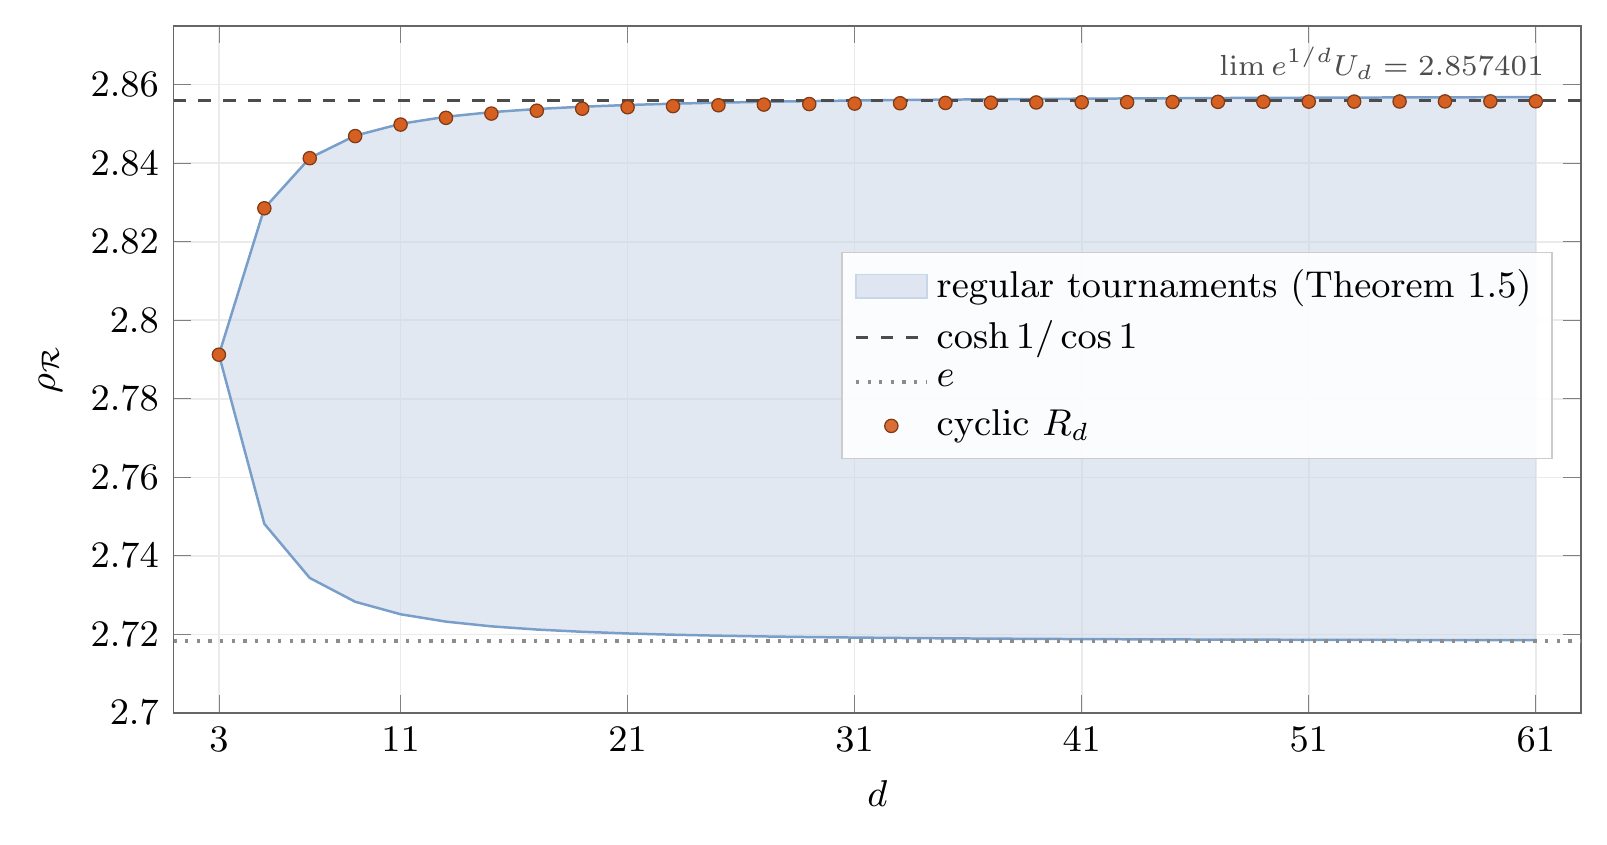
\includegraphics[width=0.86\textwidth]{figures/convergence.png}
\caption{$\rho_\cR(T)$ for regular tournaments on $d$ vertices. The dots are the cyclic tournaments $R_d$; the band is bounded by $e^{1/d}((d+1)/(d-1))^{(d-1)/2}$ and $e^{1/d}U_d$ (Theorem~\ref{thm:bounds}). The upper bound and $\rho_\cR(R_d)$ both approach the region near $\cosh1/\cos1$, while the lower bound decreases to $e$.}
\label{fig:convergence}
\end{figure}

\section{Bounds over all regular tournaments}\label{sec:bounds}

Write $s_k=\mu_k^2$. Since $\operatorname{tr}(SS^\T)=d(d-1)$ and the eigenvalues of $SS^\T=-S^2$ are $0$ and $s_1,s_1,\dots,s_m,s_m$,
\begin{equation}\label{eq:trace}
\sum_{k=1}^m s_k=\frac{d(d-1)}2,\qquad \log\rho_\cT(T)=\sum_{k=1}^m\varphi(s_k),\qquad \varphi(s)=\log\frac{d^2+s}{d^2-s}.
\end{equation}
The function $\varphi$ is strictly convex on $[0,d^2)$, since $\varphi''(s)=(d^2-s)^{-2}-(d^2+s)^{-2}>0$ for $s>0$.

\begin{lemma}\label{lem:Dd}
Let $D_d$ be the skew-symmetric $d\times d$ matrix with all entries above the diagonal equal to $1$. Its eigenvalues are $i\cot\frac{(2k-1)\pi}{2d}$, $k=1,\dots,d$; in particular its spectral radius is $\cot\frac{\pi}{2d}$.
\end{lemma}

\begin{proof}
Let $\omega^d=-1$ and $v=(1,\omega,\dots,\omega^{d-1})^\T$. Then
\[
(D_dv)_j=\sum_{l>j}\omega^{l}-\sum_{l<j}\omega^{l}=\frac{\omega^{j+1}-\omega^d}{1-\omega}-\frac{1-\omega^j}{1-\omega}=\frac{1+\omega}{1-\omega}\,\omega^j\qquad(0\le j<d),
\]
so $(1+\omega)/(1-\omega)=i\cot(\theta/2)$ is an eigenvalue for $\omega=e^{i\theta}$, $\theta=(2k-1)\pi/d$. These $d$ numbers are distinct.
\end{proof}

\begin{lemma}[Spectral radius bound]\label{lem:radiusbound}
If $B$ is a real skew-symmetric $d\times d$ matrix with $|B_{jk}|\le1$, then its spectral radius is at most $\cot(\pi/(2d))$.
\end{lemma}

\begin{proof}
The matrix $iB$ is Hermitian, so it suffices to bound $|v^*iBv|$ for every unit vector $v\in\C^d$. Changing the signs of coordinates and permuting them preserves the hypotheses on $B$ and the Rayleigh quotient. We may therefore write $v_j=r_je^{i\theta_j}$ with $r_j\ge0$ and $0\le\theta_1\le\cdots\le\theta_d<\pi$: choose the sign of each nonzero coordinate to put its argument in $[0,\pi)$ and then sort the arguments; zero coordinates may have argument zero. Then
\[
|v^*iBv|=\left|-2\sum_{j<k}B_{jk}r_jr_k\sin(\theta_k-\theta_j)\right|
\le 2\sum_{j<k}r_jr_k\sin(\theta_k-\theta_j)=|v^*iD_dv|.
\]
Every sine in the sum is nonnegative. By Lemma~\ref{lem:Dd} and the Hermitian Rayleigh bound, the last expression is at most $\cot(\pi/(2d))\|v\|^2$. This proves the claim. The bound is also recorded in~\cite[Lemma~12]{GKLV}; the proof above supplies the input used here.
\end{proof}

\begin{proof}[Proof of Theorem~\ref{thm:bounds}]
\emph{Lower bound.} By \eqref{eq:trace} and Jensen's inequality, $\log\rho_\cT(T)\ge m\,\varphi(d)=m\log\frac{d+1}{d-1}$, with equality if and only if $s_1=\dots=s_m=d$. As $S$ is normal with $S\one=0$, this happens exactly when $SS^\T=dI-J$. Expanding with $A+A^\T=J-I$ and $AJ=JA^\T=mJ$ gives
\[
SS^\T=4AA^\T+(2-d)J-I,
\]
so the equality condition is $AA^\T=\frac14\bigl((d+1)I+(d-3)J\bigl)$: every two vertices have $(d-3)/4$ common out-neighbours.

\emph{$\rho_\cR>e$.} With $x=1/d$,
\[
\log\Bigl(e^{1/d}\Bigl(\frac{d+1}{d-1}\Bigr)^m\Bigr)=x+\frac{1-x}{2x}\log\frac{1+x}{1-x}=1+\sum_{k\ge1}\frac{x^{2k}-x^{2k+1}}{2k+1}>1.
\]

\emph{Upper bound.} Lemma~\ref{lem:radiusbound} gives $s_k\le\sigma=\cot^2\frac\pi{2d}<d^2$ by Lemma~\ref{lem:Dd}. Hence $(s_1,\dots,s_m)$ lies in the polytope $\{0\le s_k\le\sigma,\ \sum s_k=d(d-1)/2\}$, on which the convex function $\sum\varphi(s_k)$ attains its maximum at a vertex. A point of the polytope with two coordinates in $(0,\sigma)$ is the midpoint of two other points of it, so at a vertex at most one coordinate lies strictly between $0$ and $\sigma$; this forces $q$ coordinates equal to $\sigma$, one further coordinate equal to $r$ when $r>0$, and all remaining coordinates equal to $0$, giving the value $\log U_d$ (also when $r=0$). As $d\to\infty$, $\sigma/d^2\to4/\pi^2$ and $d(d-1)/(2d^2)\to\frac12$; since $1<\pi^2/8<2$ we get $q=1$ for large $d$, $r/d^2\to\frac12-\frac4{\pi^2}$, and the stated limit. Finally, every limit point of $\max_T\rho_\cR(T)$ is at least $\lim\rho_\cR(R_d)=\cosh1/\cos1$ and at most $\lim e^{1/d}U_d$.
\end{proof}

\begin{table}[t]
\centering
\caption{$\rho_\cT(T)$ for the regular tournaments on $d\le9$ vertices, one row for each characteristic polynomial of $S$, from all regular tournaments on $\Z/d$ in which $0$ dominates $1,\dots,m$; ``labelled'' counts these. Every regular tournament is isomorphic to one of them. The rows come from an enumeration of these tournaments; each value in the second column is the determinant ratio of Theorem~\ref{thm:main}.}
\label{tab:small}
\renewcommand{\arraystretch}{1.12}
\begin{tabular}{@{}r>{$}r<{$}lrl@{}}
\toprule
$d$ & \rho_\cT(T) & decimal & labelled & remark\\
\midrule
5 & 44/19 & 2.315789 & 4 & $R_5$\\
\addlinespace
7 & 3032/1231 & 2.463038 & 36 & $R_7$\\
  & 3088/1287 & 2.399378 & 84 & Wormald's example\\
  & 64/27 & 2.370370 & 12 & doubly regular (Paley)\\
\addlinespace
9 & 437584/171769 & 2.547514 & 576 & $R_9$\\
  & 443488/177529 & 2.498116 & 5184 & \\
  & 5488/2197 & 2.497952 & 64 & $R_9'$ (blow-up of $R_3$)\\
  & 446656/180193 & 2.478764 & 6912 & \\
  & 446512/180337 & 2.475987 & 5184 & \\
  & 446368/180481 & 2.473213 & 1728 & \\
  & 449152/182077 & 2.466824 & 6912 & \\
  & 449008/182221 & 2.464085 & 1728 & \\
  & 449824/182857 & 2.459977 & 10368 & \\
  & 50080/20381 & 2.457191 & 5184 & \\
  & 451696/183937 & 2.455710 & 576 & circulant $\{1,2,3,5\}$\\
  & 50176/20449 & 2.453714 & 1728 & \\
\bottomrule
\end{tabular}
\end{table}

\begin{remark}\label{rem:scope}
Everything above is proved in full. Theorem~\ref{thm:main} is the exact value of Wormald's $H$ for every regular tournament, Theorem~\ref{thm:cyclic} its value and limit along the cyclic tournaments, and Theorem~\ref{thm:bounds} two bounds whose proofs use only the trace identity \eqref{eq:trace}, convexity and Lemma~\ref{lem:radiusbound}. The only inputs from outside the paper are Theorem~W, which is used in Corollary~\ref{cor:hn} and nowhere else, and the existence of doubly regular tournaments from~\cite{RB}. Table~\ref{tab:small} and the decimal values quoted in the text are computations, not theorems; the first expression in \eqref{eq:cyclic} and the exact values of Wormald's table agree for every $d\le13$ that he lists, and his decimal value $\rho_\cR(R_{81})=2.855842467\ldots$ should read $2.855842468\ldots$. The statement that $R_d$ maximises $\rho_\cT$ among regular tournaments on $d\le9$ vertices is read off from the table; for all $d$ it follows from the bound of Divoux and Wang quoted in Section~\ref{sec:intro}, and nothing else in this paper depends on it.
\end{remark}

\section*{Declarations}

\noindent\textbf{Funding.} None.

\smallskip
\noindent\textbf{Conflict of interest.} None.

\begin{thebibliography}{99}

\bibitem{AAR}
I.~Adler, N.~Alon and S.~M.~Ross, On the maximum number of Hamiltonian paths in tournaments, Random Structures Algorithms 18 (2001), no.~3, 291--296. \href{https://doi.org/10.1002/rsa.1010}{doi:10.1002/rsa.1010}.

\bibitem{Al}
N.~Alon, The maximum number of Hamiltonian paths in tournaments, Combinatorica 10 (1990), no.~4, 319--324. \href{https://doi.org/10.1007/BF02128667}{doi:10.1007/BF02128667}.

\bibitem{Bha22a}
D.~Bhattacharjee, Establishing equivariant class $[O]$ for hyperbolic groups, Asian Res. J. Math. 18 (2022), no. 11, 362--369. \href{https://doi.org/10.9734/arjom/2022/v18i11615}{doi:10.9734/arjom/2022/v18i11615}.

\bibitem{Bha22b}
D.~Bhattacharjee, Non-commutativity over canonical suspension $\eta$ for genus $g\ge1$ in hypercomplex structures for potential $\rho\phi$, Asian Res. J. Math. 18 (2022), no. 11, 332--341. \href{https://doi.org/10.9734/arjom/2022/v18i11607}{doi:10.9734/arjom/2022/v18i11607}.

\bibitem{BB26}
D.~Bhattacharjee, U.~Bhattacharya, Iterated nerve complexes for $k$-fold sensor coverage, Preprints.org (2026). \href{https://doi.org/10.20944/preprints202606.1351.v2}{doi:10.20944/preprints202606.1351.v2}.

\bibitem{DW}
A.~Divoux and S.~Wang, The maximum number of Hamiltonian cycles in tournaments, preprint, \href{https://arxiv.org/abs/2610.23755}{arXiv:2610.23755} (2026).

\bibitem{FK}
E.~Friedgut and J.~Kahn, On the number of Hamiltonian cycles in a tournament, Combin. Probab. Comput. 14 (2005), no.~5--6, 769--781. \href{https://doi.org/10.1017/S0963548305006863}{doi:10.1017/S0963548305006863}.

\bibitem{GKLV}
A.~Grzesik, D.~Kr\'al', L.~M.~Lov\'asz and J.~Volec, Cycles of a given length in tournaments, J. Combin. Theory Ser. B 158 (2023), 117--145. \href{https://doi.org/10.1016/j.jctb.2022.07.007}{doi:10.1016/j.jctb.2022.07.007}.

\bibitem{RB}
K.~B.~Reid and E.~Brown, Doubly regular tournaments are equivalent to skew Hadamard matrices, J. Combin. Theory Ser. A 12 (1972), no.~3, 332--338. \href{https://doi.org/10.1016/0097-3165(72)90098-2}{doi:10.1016/0097-3165(72)90098-2}.

\bibitem{Sz}
T.~Szele, Kombinatorikai vizsg\'alatok az ir\'any\'itott teljes gr\'affal kapcsolatban, Mat. Fiz. Lapok 50 (1943), 223--256.

\bibitem{W}
N.~C.~Wormald, Tournaments with many Hamilton cycles, preprint, on the author's web page since 2013; \href{https://arxiv.org/abs/2610.16245}{arXiv:2610.16245} (2026).

\end{thebibliography}

\end{document}
